\section{Mechanischer Aufbau} \label{Mechanischer_Aufbau}
	Die mechanische Konstruktion wurde so einfach wie möglich gestaltet, um in erster Linie das schnelle Testen der Software zu ermöglichen. Der Aufbau besteht aus zwei Kunststoffplatten, einem Verbindungsblech und vier Stiften, welche miteinander verbunden werden sollen. 
	\\
	Der Montageprozess erfolgt in drei Schritten: Zunächst werden die beiden Platten miteinander verbunden (Abb. \ref{fig:Montageschritt 1}). Dafür sind sie mit «Fingerzinkungen» ausgestattet, durch die sie ineinandergesteckt werden. Anders als im ursprünglichen Konzept vorgesehen, bei dem eine Eckverbindung angedacht war (Abb. \ref{fig:Teilprozesse}), liegen die Platten in einer Ebene. Erste Simulationen mit der Software «RoboDK» ergaben, dass eine Umsetzung mit Eckverbindung die Erreichbarkeit der verschiedenen Positionen für den Roboter deutlich erschwert hätte. Durch den montierten Kraftsensor und Greifer wird der \Gls{TCP} versetzt, wodurch der Arbeitsbereich des Roboters zusätzlich eingeschränkt wird. Die flache Anordnung der Platten erleichtert die Zugänglichkeit erheblich, während der grundlegende Prozess unverändert bleibt.
	\\
	Im zweiten Schritt wird das Verbindungsblech auf die zusammengefügten Platten aufgelegt (Abb. \ref{fig:Montageschritt 2}). Es muss dabei exakt auf die Lochpositionen der Platten ausgerichtet werden. Im dritten Schritt werden die Platten und das Blech mithilfe von Stiften fixiert (Abb. \ref{fig:Montageschritt 3}). Die Stifte werden in die vorgesehenen Löcher gedrückt, wobei eine enge, aber noch als Spielpassung definierte Toleranz vorliegt. Der Roboter muss dabei äusserst präzise arbeiten und in der Lage sein, eine Verkantung zu erkennen. Auf Verfahren wie Schrauben oder Nieten wurde bewusst verzichtet, um den Einsatz eines spezifischen Werkzeugs für den Roboter zu vermeiden.
	
	 \begin{figure}[h!]
		\centering
		\begin{subfigure}[b]{0.3\textwidth}
			\centering
			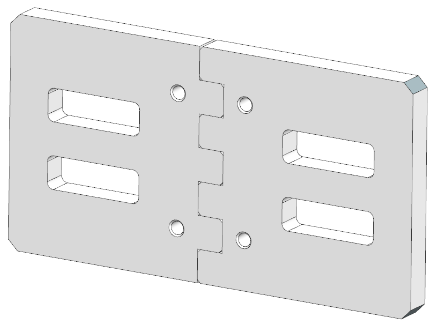
\includegraphics[width=\textwidth]{04_Anwendung_und_Aufbau/Montageschritt_1}
			\caption{Montageschritt 1}
			\label{fig:Montageschritt 1}
		\end{subfigure}
		\hfill
		\begin{subfigure}[b]{0.3\textwidth}
			\centering
			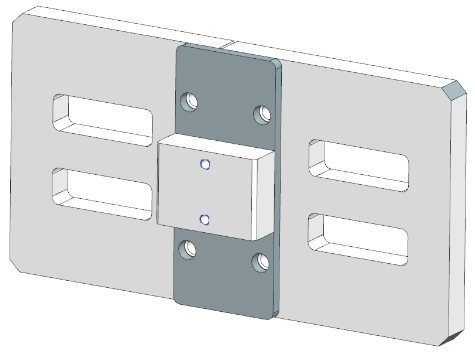
\includegraphics[width=\textwidth]{04_Anwendung_und_Aufbau/Montageschritt_2}
			\caption{Montageschritt 2}
			\label{fig:Montageschritt 2}
		\end{subfigure}
		\hfill
		\begin{subfigure}[b]{0.3\textwidth}
			\centering
			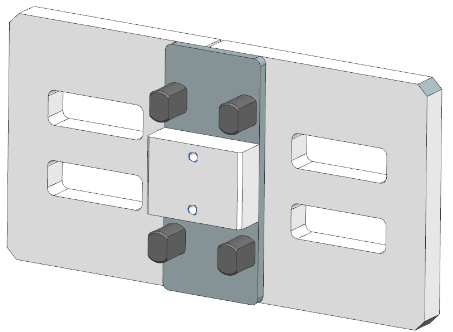
\includegraphics[width=\textwidth]{04_Anwendung_und_Aufbau/Montageschritt_3}
			\caption{Montageschritt 3}
			\label{fig:Montageschritt 3}
		\end{subfigure}
		\caption{Anwendungsteilprozesse}
		\label{fig:Montageschritte}
	\end{figure}
	
	\begin{bfhNoteBox}
		Alle Detailzeichnungen in Fertigungsdaten werden im Anhang beigelegt. 
	\end{bfhNoteBox}	
	
	\vspace{5mm} 

	Die Montage wird auf einer Platte durchgeführt. Gleichzeitig dient die Platte auch als Halterung für die Komponenten (Abb. \ref{fig:Montagevorrichtung}). Im unteren linken Bereich werden die Platten miteinander montiert. Damit eine Referenzposition sichergestellt werden kann, dient ein L-Stück als Anschlag. Die erste Platte wird damit in X- und Y-Richtung positioniert. Das Ziel ist, dass der Roboter den Anschlag durch den Kraftsensor erkennt und entsprechend die Bewegung stoppt.
	
	\newpage
	
	Der UR5 wird mit einem Kraftsensor und einem Greifer ausgestattet (Abb. \ref{fig:AnlageReal}). Der Kraftsensor wird am UR5 montiert, während der Greifer am Kraftsensor befestigt wird. Um die Verbindung zwischen dem Kraftsensor und dem UR5 herzustellen, wurde eine Adapterplatte entwickelt. Der Greifer hingegen kann direkt am Sensor befestigt werden, ohne dass ein zusätzlicher Adapter erforderlich ist. Für ein präzises und zuverlässiges Greifen der Anwendungsteile wurden spezielle Backeneinsätze für den Greifer konstruiert.
	
	 \begin{figure}[h!]
		\centering
		\begin{subfigure}[b]{0.6\textwidth}
			\centering
			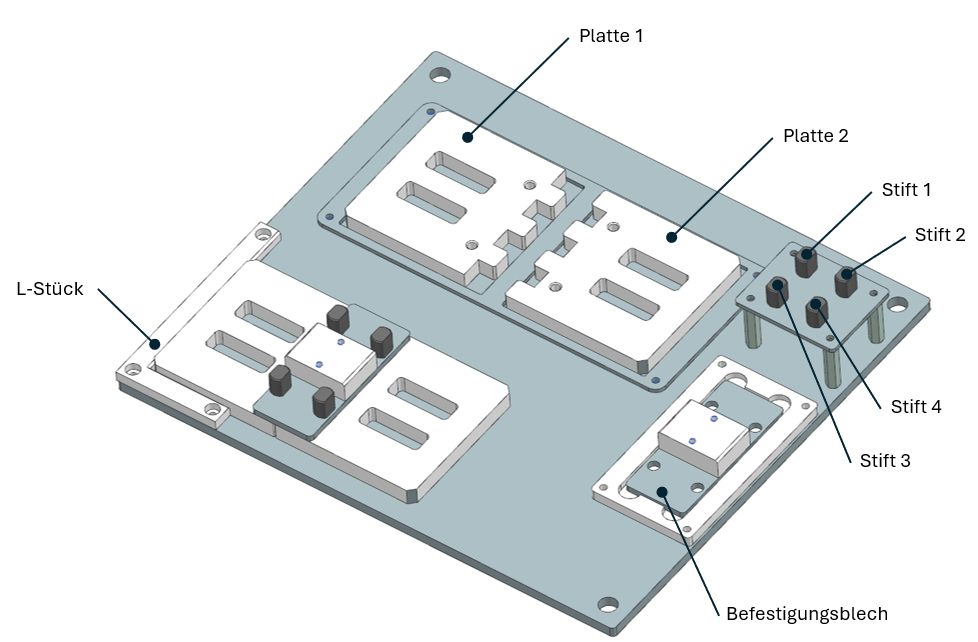
\includegraphics[width=\textwidth]{04_Anwendung_und_Aufbau/Montagevorrichtung}
			\caption{Montagevorrichtung}
			\label{fig:Montagevorrichtung}
		\end{subfigure}
		\hfill
		\begin{subfigure}[b]{0.35\textwidth}
			\centering
			\includegraphics[width=\textwidth]{09_Auswertung/AnlageReal}
			\caption{Realer Aufbau der Anlage}
			\label{fig:AnlageReal}
		\end{subfigure}
		\caption{Umgesetzte Anwendung}
		\label{fig:AnwendungUmgesetzt}
	\end{figure}
	
	Mit der Fertigung und Montage des mechanischen Aufbaus, kann in einem nächsten Schritt mit der Umsetzung der Software begonnen werden. 

	
	